\title{\textbf{H a t c h} - A Python Preprocessor}

\author{
	\textbf{Addison Boyer} \\
	\textit{Natural Language Processing} \\
	\textit{Spring 2020}
}

\date{}

\documentclass[12pt]{article}
\usepackage{graphicx}
\usepackage{listings}
\usepackage{color}

\definecolor{dkgreen}{rgb}{0,0.6,0}
\definecolor{gray}{rgb}{0.5,0.5,0.5}
\definecolor{mauve}{rgb}{0.58,0,0.82}


\lstset{frame=tb,
  language=Python,
  aboveskip=3mm,
  belowskip=3mm,
  showstringspaces=false,
  columns=flexible,
  basicstyle={\small\ttfamily},
  numbers=none,
  numberstyle=\tiny\color{gray},
  keywordstyle=\color{blue},
  commentstyle=\color{dkgreen},
  stringstyle=\color{mauve},
  breaklines=true,
  breakatwhitespace=true,
  tabsize=3
}

\begin{document}
\maketitle
\begin{center}
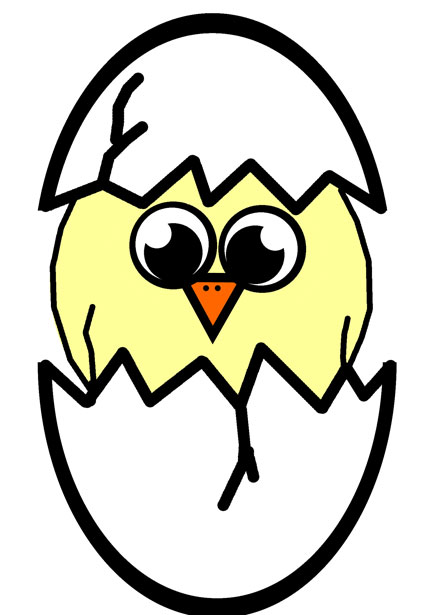
\includegraphics[scale=0.45]{../images/hatchchick.JPG}
\end{center}
\pagebreak

\section{Getting Started}
\paragraph{} All Hatch statements begin with a special Hatch comment identifier (\textbf{\#!}).  If the Hatch comment identifier is not present, the line will be treated as interpretable Python code.  All lines beginning with \textbf{\#!} will ``hatch'' into interpretable Python code, given the correct Hatch syntax.

\section{Keywords}
\begin{enumerate}
\item{\textbf{class}}
- Used to define a Python class in Hatch.
\item{\textbf{get}}
- Used to define an attributes getter/getters in Hatch.
\item{\textbf{set}}
- Used to define an attributes setter/setters in Hatch.
\item{\textbf{str}}
- Used to define a classes toString() method in Hatch.
\item{\textbf{hatch()}}
- Used to exit a Hatch interactive shell.
\end{enumerate}

\section{The Hatch Egg}
\paragraph{}The Hatch egg is where parameter and attribute names are passed.  An egg consists of a comma delimited list of variable names surrounded by parenthesis.  An empty hatch egg will result in the following error: \textit{Empty egg to be hatched, aborting..}

\section{Syntax}
\begin{enumerate}
\item{\textbf{Class Declarations}} \\ \\
\#! class Person = (name, age, ...)
\item{\textbf{Getter Declarations}} \\ \\
\#! get = (name, age, ...)
\item{\textbf{Setter Declarations}} \\ \\
\#! set = (name, age, ...)
\item{\textbf{toString() Declarations}} \\ \\
\#! str = (name, age, ...)
\item{\textbf{Variable Declarations}} \\ \\
\#! name = `Addison' \\ \\
\#! age = 20 \\ \\
\#! age = 20.0 \\ \\
\end{enumerate}


\section{Hello Hatch}

\begin{lstlisting}
# HelloHatch.Hatch
import sys

#! class HelloHatch = (hello, hatch)
	#! get = (hello, hatch)
	#! set = (hello, hatch)
	#! str = (hello, hatch)

def main(argv):

	hello_hatch = HelloHatch("Hello", "Hatch!")
	print(hello_hatch)
	
if(__name__ == "__main__"):
	main(sys.argv[1:])

\end{lstlisting}
\textbf{make -B} \\
\textbf{./interpreter.out HelloHatch.Hatch $>$ HelloHatch.py} \\

\pagebreak
\begin{lstlisting}
# HelloHatch.py
import sys

     
class HelloHatch(object):
	def __init__(self,hello,hatch):
		self.hello = hello
		self.hatch = hatch

    
	def get_hello(self):
		return self.hello
	def get_hatch(self):
		return self.hatch

    
	def set_hello(self,hello):
		self.hello = hello
	def set_hatch(self,hatch):
		self.hatch = hatch

    
	def __str__(self):
		return str(self.hello) + ' ' + str(self.hatch)


def main(argv):

	hello_hatch = HelloHatch("Hello", "Hatch!")
	print(hello_hatch)

if(__name__ == "__main__"):
	main(sys.argv[1:])
\end{lstlisting}

\textbf{python3 HelloHatch.py} \\

Hello Hatch!



\end{document}
